% Modelo de relatório no estilo artigo em duas colunas
\documentclass[twocolumn]{article}
\usepackage[utf8]{inputenc}
\usepackage{amsmath}
\usepackage{subcaption}
\usepackage{mathtools}
\usepackage{graphicx}
\usepackage{color}
\usepackage{authblk}
\usepackage{lmodern}
% \usepackage[colorlinks,citecolor=black,urlcolor=black,bookmarks=false,hypertexnames=true]{hyperref}
\usepackage[margin=0.9in]{geometry}
\usepackage{pdfpages}
\usepackage{fancyhdr}
\usepackage[utf8]{inputenc}

\usepackage[sorting=none,style=numeric]{biblatex}
\addbibresource{refs.bib}
\usepackage[justification=centering]{caption}
\usepackage{makecell}
\usepackage{booktabs}
\usepackage{hhline}
\usepackage{amsmath}
\usepackage{amssymb}
\usepackage{soul}
\usepackage{gensymb}
\usepackage{listings}

\setlength\parindent{0pt}


\newcommand{\myname}{Nishant Aswani}
\newcommand{\mynetid}{nsa325}
\newcommand{\myemail}{nsa325@nyu.edu}
\newcommand{\myhwtype}{Lab }
\newcommand{\myhwnum}{10}
\newcommand{\mycoursenumber}{ENGR-UH 3511}
\newcommand{\myclassname}{Computer Organization and Architecture}
\newcommand{\myassignmenttitle}{Out-of-Order Execution}
\newcommand{\myinstructor}{Cristoforos Vasilatos}

\newcommand{\cc}[1]{\texttt{#1}}

\lstset{
  basicstyle=\ttfamily,
  escapeinside=||
}

% Tamanho das margens:
% \geometry{
% 	a4paper,
% 	total={170mm,257mm},
% 	left=30mm,
% 	top=20mm,
% }
%%%%%%%%%%%%%%%%%%%%%%%%%%%%%%%%%%%%%%%%%
% Bibliografia estilo ABNT. Se não tiver instalado, comente a linha abaixo.
% \usepackage[alf, abnt-etal-list=0, abnt-emphasize=bf,abnt-last-names=bibtex, abnt-etal-text=it, abnt-etal-cite=2]{abntex2cite}
%%%%%%%%%%%%%%%%%%%%%%%%%%%%%%%%%%%%%%%%%

% Dados de identificação
\title{\myassignmenttitle}
\author{\myname, \myemail}
\affil{\myclassname (\mycoursenumber), Instructor \myinstructor}
\date{}

\begin{document}
%%%%%%%%%%%%%%%%%%%%%%%%%%%%%%%%%%%%%%%%%%%%%%%% COVER PAGE %%%%%%%%%%%%%%%%%%%%%%%%%%%%%%%%%%%%%%%%%%%%%%%%%%%%
\onecolumn
\pagestyle{fancy}
\fancyhf{}
\renewcommand{\headrulewidth}{0pt}
\rhead{\textbf{Division of Engineering}}
\lhead{\textbf{NYU Abu Dhabi}}

\begin{center}
  
\includegraphics[scale=0.15]{etc/NYUAD-alt-logo.jpg}
\end{center}

{\vspace{2.5em}}

\begin{center}
    \Huge{\textbf{\mycoursenumber}}\\
    {\vspace{0.5em}}
    \Huge{\textbf{\myclassname}}
\end{center}

{\vspace{10em}}

\begin{center}
  \begin{tabular}{|rp{5.0cm}lll|}
    \hline
    &  &  &  & \\
    &  &  &  & \\
    \Large{\textbf{Name:}} & \Large{\myname}
    
    \  &  &  & \\
    \Large{\textbf{Net ID:}} & \Large{\mynetid}
    
    \  &  &  & \\
    \Large{\textbf{Assignment Title:}} & \Large{\myhwtype \myhwnum}
    
    \
    
    \  &  &  & \\
    \hline
  \end{tabular}
\end{center}

\

{\newpage}
%%%%%%%%%%%%%%%%%%%%%%%%%%%%%%%%%%%%%%%%%%%%%%%% COVER PAGE %%%%%%%%%%%%%%%%%%%%%%%%%%%%%%%%%%%%%%%%%%%%%%%%%%%%

\maketitle        

% Resumo de no máximo 200 palavras
% \begin{abstract}
% Este documento orienta a descrição das atividades práticas desenvolvidas em laboratório. São usados como exemplo conceitos da Aula 01 de Acionamentos Elétricos sobre partida direta de motor de indução trifásico. Nesta atividade, um motor é acionado com conexões estrela e triângulo a vazio. As correntes nominais e de partida são medidas com amperímetro analógico e comparadas entre si. Nota-se que, mesmo sem carga, as corrente em estrela são maiores. 
% \end{abstract}

\section{Introduction}

Out-of-order execution executes instructions in a different order than in which they were fed into the processor. The purpose of out of order execution is to execute instructions based on availability on data and reduce idle time.

\section{Performance Optimization Configurations}

For this lab, \cc{mplat, itlb, \& dtlb}, were left on their respective default values.


\subsection{Default Conditions}

We clearly see that using default conditions, the processor has better performance with out-of-order execution


\begingroup
    \centering
    \medskip
    %width=\columnwidth
    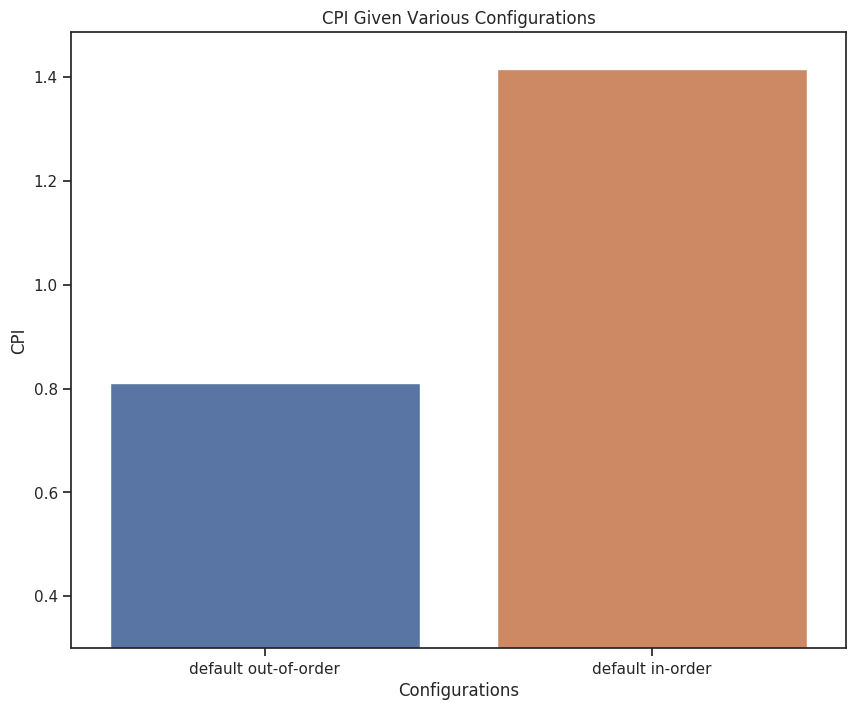
\includegraphics[width=0.6\columnwidth]{Lab-Tex/LabX-images/default.png}
    \captionof{figure}{CPI comparison with default processor conditions and execution order}
    \label{fig:lsq}
    \medskip
\endgroup

\begingroup
    \medskip
    \centering
    \def\arraystretch{1.5}
        \begin{tabular}{cc}
            \toprule
            Order & CPI\\
             \midrule
            In-order & 1.4155\\
            Out-of-order & 0.8102\\
            \bottomrule
        \end{tabular}
    \captionof{table}{Default configurations with different order executions}
    \label{table:btb}
\endgroup

\subsection{Varying \cc{fpalu}, \cc{ialu}, and \cc{fpmult}}

We would assume that increasing the number of arithmetic logic units (ALUs) or multipliers would significantly improve the performance of the processor. There are 4 \cc{fpalus} and \cc{ialus}, and 1 \cc{fpmult} by default. No tested combination of these three execution components improved performance.

\begingroup
    \medskip
    \centering
    \def\arraystretch{1.5}
        \begin{tabular}{ccccc}
            \toprule
            Order & CPI & # of \cc{ialu} & # of \cc{fplu} & # of \cc{fpmult}\\
             \midrule
            In-order & 1.4155 & 4 & 4 & 1\\
            Out-of-order & 0.8102 & 4 & 4 & 1\\
            \midrule
            In-order & 1.4155 & 8 & 8 & 1\\
            Out-of-order & 0.8102 & 8 & 8 & 1\\
            \midrule
            In-order & 1.4155 & 4 & 8 & 8\\
            Out-of-order & 0.8102 & 4 & 8 & 8\\
            \bottomrule
        \end{tabular}
    \captionof{table}{Adding ALUs to different order executions}
    \label{table:btb}
\endgroup

\subsection{Varying queue sizes}

The load/store queue is a microarchitecture concept used to keep track of load and store instructions within a processor to aid in execute these instructions out-of-order. The instruction queue size determines the number of instructions that are loaded in at once in the processor. 

\begingroup
    \centering
    \def\arraystretch{1.5}
        \begin{tabular}{cccc}
            \toprule
            Order & CPI & \cc{ifqsize} & \cc{lsqsize}\\
             \midrule
            In-order & 1.4155 & 4 & 8\\
            Out-of-order & 0.8102 & 4 & 8\\
            \midrule
            In-order & 1.4221 & 4 & 2\\
            Out-of-order & 1.1644 & 4 & 2\\
            \bottomrule
        \end{tabular}
    \captionof{table}{Decreasing lsq size for different order executions}
    \label{table:btb}
\endgroup

We see that a drastic change in the \cc{lsqsize} has a negative effect on performance, especially for the out-of-order secheme. We can then infer that the lsq is an import microarchitecture designed for the out-of-order scheme, which makes sense since there would be little use to keep track of load and store operations if they were carried out in-order. In fact, one may have hypothesized that decreasing the \cc{lsq} would have no effect on the in-order scheme. 

\begingroup
    \centering
    \medskip
    %width=\columnwidth
    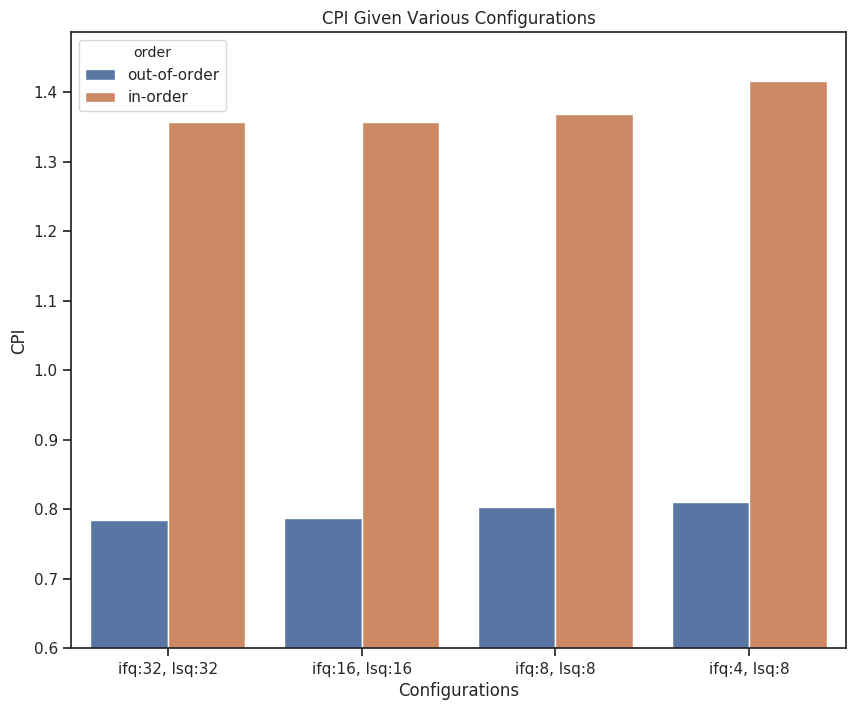
\includegraphics[width=0.6\columnwidth]{Lab-Tex/LabX-images/queue.png}
    \captionof{figure}{CPI comparison with varying queue sizes for different execution orderf}
    \label{fig:}
    \medskip
\endgroup

\begingroup
    \medskip
    \centering
    \def\arraystretch{1.5}
        \begin{tabular}{cccc}
            \toprule
            Order & CPI & \cc{ifqsize} & \cc{lsqsize}\\
             \midrule
            In-order & 1.4155 & 4 & 8\\
            Out-of-order & 0.8102 & 4 & 8\\
            \midrule
            In-order & 1.3691 & 8 & 8\\
            Out-of-order & 0.8034 & 8 & 8\\
            \midrule
            In-order & 1.3572 & 16 & 16\\
            Out-of-order & 0.7871 & 16 & 16\\
            \midrule
            In-order & 1.3571 & 32 & 32\\
            Out-of-order & 0.7851 & 32 & 32\\
            \bottomrule
        \end{tabular}
    \captionof{table}{Varying ifqsize and lsqsize for different order executions}
    \label{table:btb}
\endgroup

\subsection{Varying queue size in conjunction with ALU and mult units}

Earlier, we saw that varying the number of ALU and mult units alone had little effect on the performance. \\

\begingroup
    \centering
    \def\arraystretch{1.5}
        \begin{tabular}{cccccc}
            \toprule
            Order & CPI & \cc{ifqsize} & \cc{lsqsize} & \cc{fpalu} & \cc{fpmult}\\
            \midrule
            In-order & 1.3572 & 16 & 16 & 4 & 1\\
            Out-of-order & 0.7871 & 16 & 16 & 4 & 1\\
            \midrule
            In-order & 1.3572 & 16 & 16 & 8 & 4\\
            Out-of-order & 0.7871 & 16 & 16 & 8 & 4\\
            \bottomrule
        \end{tabular}
    \captionof{table}{Varying fpalu and fpmult for different order executions}
    \label{table:btb}
\endgroup

Once again, we see that increasing the ALU and mult units has no performance improvement.

\subsection{Varying issue width with ALU and mult units}

Rather than blindly vary parameters in hopes to improve performance, some reading was done to make a more educated guess. It was realized that improving the capacity (queue) and parallel processing power (ALU and mult units) is worthless if the processor cannot take in more instructions at once. Hence, the best configuration so far was used as the baseline to then vary the issue width. \\

\begingroup
    \medskip
    \centering
    \def\arraystretch{1.5}
        \begin{tabular}{cccccccc}
            \toprule
            Order & CPI & \cc{ifqsize} & \cc{lsqsize} & \cc{fpalu} & \cc{fpmult} & \cc{issue width}\\
            \midrule
            In-order & 1.3571 & 32 & 32 & 8 & 4 & 4\\
            Out-of-order & 0.7851 & 32 & 32 & 8 & 4 & 4\\
            \midrule
            In-order & 1.3571 & 32 & 32 & 8 & 4 & 8\\
            Out-of-order & 0.7735 & 32 & 32 & 8 & 4 & 8\\
            \midrule
            In-order & 1.3571 & 32 & 32 & 8 & 4 & 16\\
            Out-of-order & 0.7735 & 32 & 32 & 8 & 4 & 16\\
            \bottomrule
        \end{tabular}
    \captionof{table}{Varying ifqsize and lsqsize for different order executions}
    \label{table:btb}
    \medskip
\endgroup

Although we see a decrease in CPI, this decrease was capped once we increased issue width to 16. Naturally, the next parameter to tune was the commit width. \\

\begingroup
    \medskip
    \centering
    \def\arraystretch{1.5}
        \begin{tabular}{cccccccc}
            \toprule
            Order & CPI & \cc{ifqsize} & \cc{lsqsize} & \cc{fpalu} & \cc{fpmult} & \cc{issue width} & \cc{commit width}\\
            \midrule
            In-order & 1.3571 & 32 & 32 & 8 & 4 & 4 & 4\\
            Out-of-order & 0.7851 & 32 & 32 & 8 & 4 & 4 & 4\\
            \midrule
            In-order & 1.3571 & 32 & 32 & 8 & 4 & 8 & 4\\
            Out-of-order & 0.7735 & 32 & 32 & 8 & 4 & 8 & 4\\
            \midrule
            In-order & 1.3571 & 32 & 32 & 8 & 4 & 16 & 4\\
            Out-of-order & 0.7735 & 32 & 32 & 8 & 4 & 16 & 4\\
            \midrule
            In-order & 1.3571 & 32 & 32 & 8 & 4 & 16 & 8\\
            Out-of-order & 0.7728 & 32 & 32 & 8 & 4 & 16 & 8\\
            \bottomrule
            In-order & 1.3571 & 32 & 32 & 8 & 4 & 16 & 16\\
            Out-of-order & 0.7728 & 32 & 32 & 8 & 4 & 16 & 16\\
            \bottomrule
        \end{tabular}
    \captionof{table}{Varying ifqsize and lsqsize for different order executions}
    \label{table:btb}
\endgroup

We make a final attempt by increasing all of the parameters that seem to have contributed to a lower out-of-order execution time:

\begingroup
    \medskip
    \centering
    \def\arraystretch{1.5}
        \begin{tabular}{cccccccc}
            \toprule
            Order & CPI & \cc{ifqsize} & \cc{lsqsize} & \cc{fpalu} & \cc{fpmult} & \cc{issue width} & \cc{commit width}\\
            \midrule
            In-order & 1.4155 & 4 & 8 & 8 & 4 & 1 & 4\\
            Out-of-order & 0.8102 & 4 & 8 & 8 & 4 & 1 & 4\\
            \midrule
            In-order & 1.3571 & 4 & 8 & 8 & 4 & 1 & 4\\
            Out-of-order & 0.7696 & 4 & 8 & 8 & 4 & 1 & 4\\
            \bottomrule
        \end{tabular}
    \captionof{table}{Varying ifqsize and lsqsize for different order executions}
    \label{table:btb}
\endgroup


\section{Discussion and Conclusion}

Essentially, we see that increasing the performance of the CPU processor in the case of out-of-order execution requires the tuning of several parameters. The idea is that providing an abundance of one kind of resource, as we saw in Section 2.2, can have little to no effect. This is because there may be bottlenecks at a different section of the processor that do not allow for the use of these extra resources. \\

In the case of the queue sizes, it simply varying the queue sizes helped because that was most likely the bottleneck in the default configuration. We see that the previous observation still stands in the case of varying the issue width, because there was a ceiling hit once we increase the issue width but not the commit width. It is not necessary that in any given configuration there is a single bottleneck, hence varying multiple parameters can also have the effect of increasing performance. \\

We also see that after a certain point, there is no benefit to the in-order processor. It seems that only the queue sizes affected the CPI of the in-order processor. We can assume that all other components built for the out-of-order architecture would not provide any improvements as well. In regards to whether it is worth having all of these extra components for the improvement of CPI is a matter of cost.\\

As usual, there is a likely middle ground that does not max out the queue sizes, instruction commit/issue widths, # of execution units, etc., but still provides a good performance improvement. As an example, we see in Figure \ref{fig:lsq} that increasing the instruction fetch queue from the default size 4 to 8 has a relatively large improvement for in-order CPI, but further increase in size provides diminishing returns. On the other hand, we may choose to not increase the instruction fetch queue size for an out-of-order scheme because the improvement is not as great. Given a budget, we may be able to vary a different parameter that provides a larger improvement in CPI.\\

Overall, of course the out-of-order processor severely outperforms the in-order processor because it is designed to reduce stalls in the pipeline. Tuning these parameters further improves the performance because it gives the processor more space to handle and reorder a greater number of instructions at once, potentially decreasing more stalls in a given program. \\











%%%%%%%%%%%%%%%%%%%%%%%%%%5
% BIBLIOGRAFIA 
% Estilo de bibliografia ABNT. Se não tiver instalado, mude para plain ou ieeetr

%\bibliographystyle{plain} % Inclua isso se não tiver ABNTEX instalado
% \begin{thebibliography}{refs}
% \bibitem{}
\printbibliography
% \end{thebibliography}
\end{document}